%!TEX root = ../main.tex
\chapter{Experiments}\label{chap:experiments}
\section{Workflow}\label{sec:workflow}

本節では、実環境データを対象にした、屈折を考慮した水中3次元再構成のための完全なパイプラインを概説する。

\begin{figure}[htbp]
  \centering
  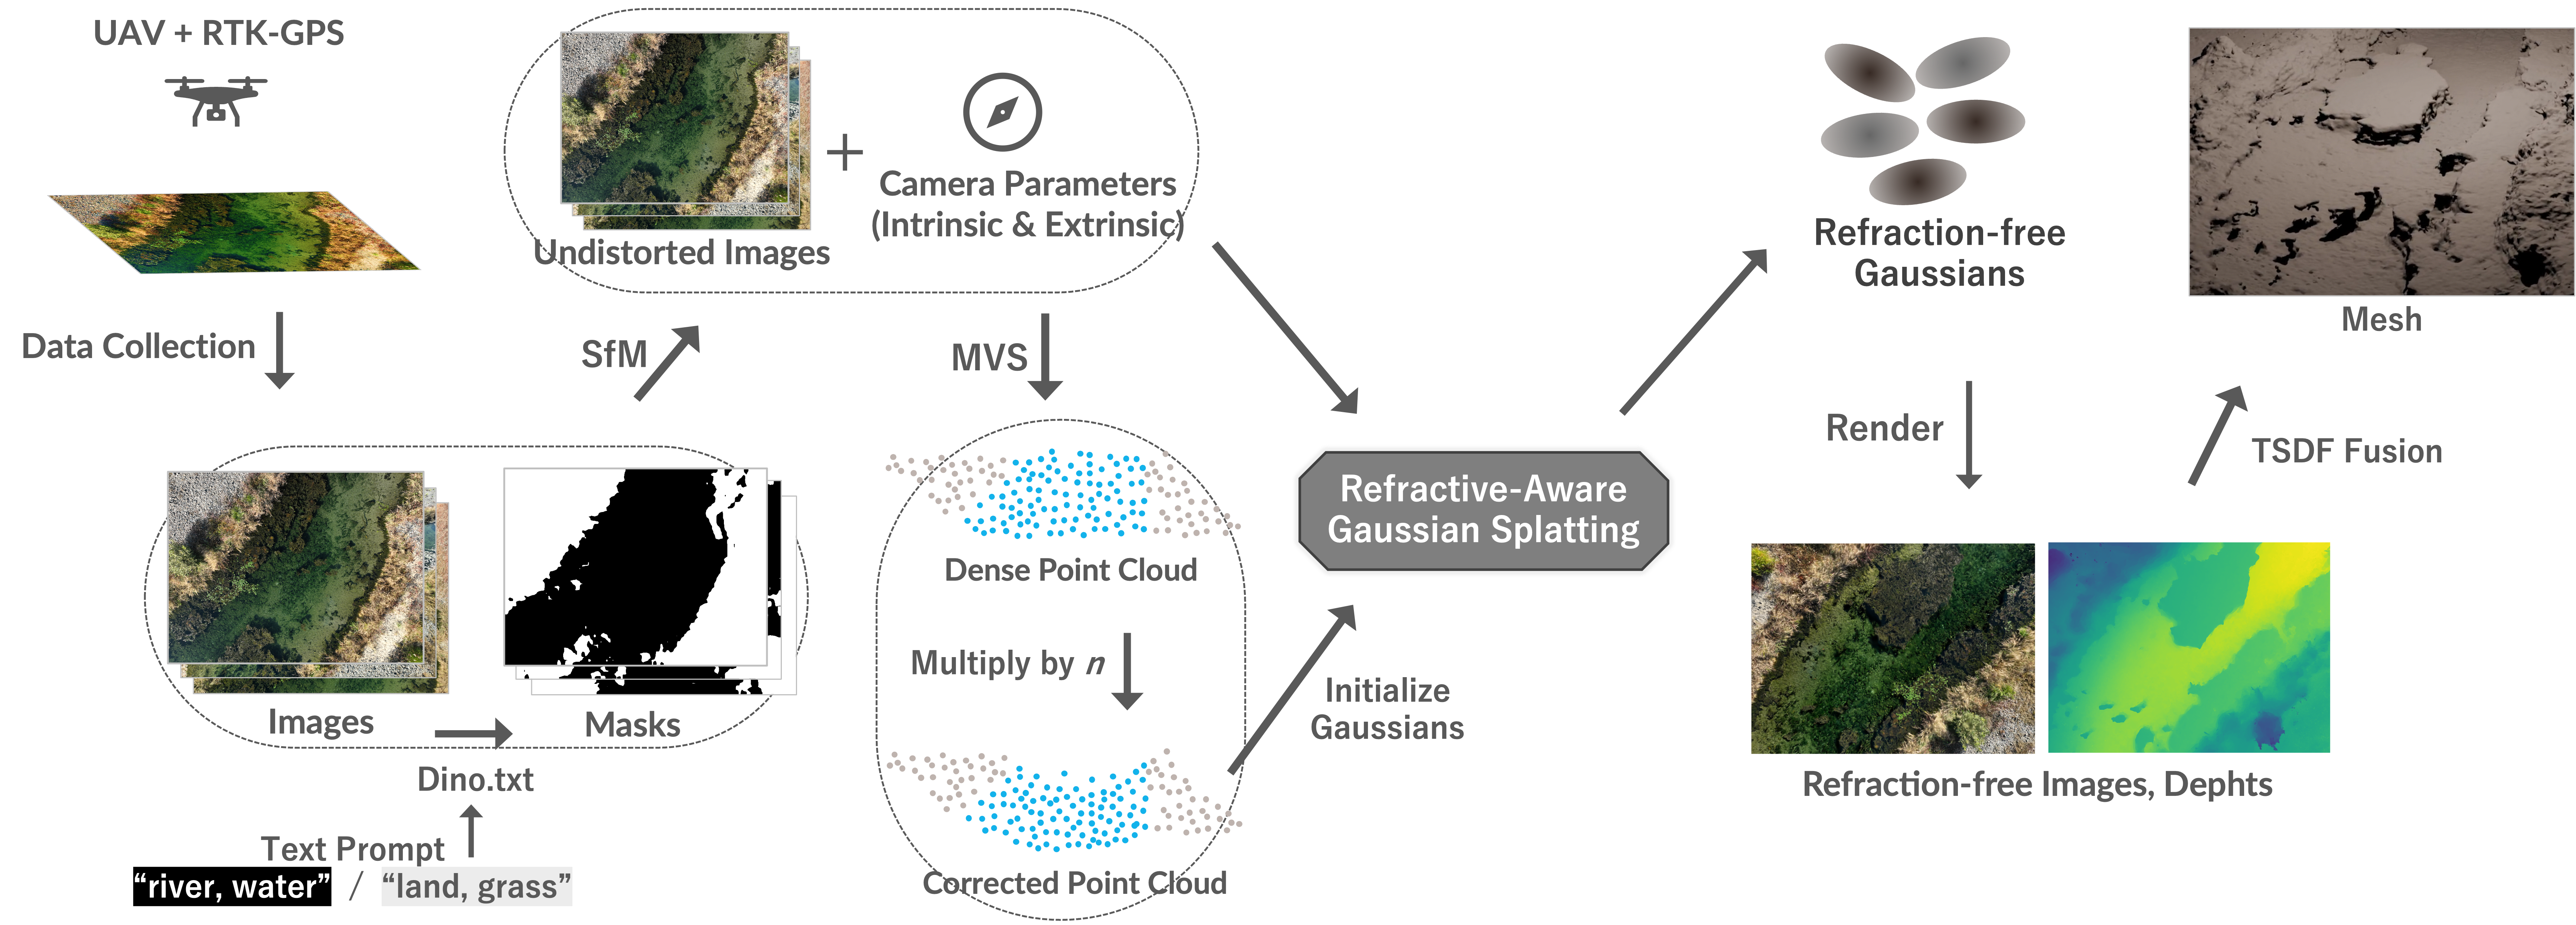
\includegraphics[width=0.95\textwidth]{figure/70_experim/workflow.png}
  \caption{
    実環境データを対象にした、屈折を考慮した水中3次元再構成のための完全なパイプライン。
    }
    \label{fig:workflow}
\end{figure}


\subsection{データ収集とセマンティック・セグメンテーション}\label{subsec:data-acquisition}

\subsubsection{UAVによる画像取得とジオリファレンス}

RTK-GPS(Real-Time Kinematic GPS)を搭載したUAVを用いて、河川および陸地を含む対象領域を撮影する。
各画像には、RTK測位による高精度なカメラ外部パラメータ(緯度・経度・高度)がメタデータとして付与される。
これにより、SfMにおいての拘束条件を追加し、実スケールでの再構成精度を保証する。
\note{Field Studyの具体的な詳細は前章ののDatasetで}

\subsubsection{Vision-Language Modelによるマスク生成}

RA-GSは、入力として正確なカメラ内部・外部パラメータを期待する。
これらは既存のパイプラインと同様\cite{Kerbl2023ToG_3DGS,Schonberger2016ECCV_PatchMatchStereo}に、SfMを用いて推定する。
屈折面が存在することで、SfM前提の光の直進性が成立しなくなり、精度は悪化し、また、屈折の影響の大きいシーンでは特徴点のRANSACによる整合ができなくなる場合も考えれる。
そこで、SfMに入力画像とその除外エリアを示すマスク画像を入力する。
これは、一般のシーンの三次元復元でも一般的な手法であり、陸域であれば、人物や車両などの移動体、鏡などの反射物を除外する。
本研究での結果は商用フォトグラメトリソフトであるRealityScan\cite{RealityScan}を使用したが、COLMAPや他のフォトグラメトリソフトウェアでも同様の手法が実現可能である。

この手法では、画像の取得で常に十分な陸域を含める必要があり、UAVの高度や角度に関しての柔軟性を失う。
後述するように、RA-GSでは、カメラ外部パラメータに関しての勾配も追跡可能で、Photometricな情報からのカメラポーズ推定も可能である。
外部パラメータの初期値にはGPSによるジオリファレンスとドローンのログデータによる姿勢方角情報を使用する。
現在は内部パラメータまでの最適化はできないため、予めカメラはキャリブレーションを行い、歪み補正を行っておく。
また、R-SfM\cite{Makris2024_refractive-aware-sfm}を用いて、屈折領域込みでのカメラポーズ推定も可能である。
\note{現在Codeも公開されているが、正直いい実装には思えなかった。}


\begin{figure}[htbp]
  \centering
  \includegraphics[width=0.95\textwidth]{figure/70_experim/DinoTXT.png}
  \caption{
    Dino.txtの概要。
    \cite{Jose2025CVPR_DINOv2-Text}から引用。
    (左):DinoV2\cite{Oquab2023_DINOv2}による自己教師あり学習(Self-Supervised Learning: SSL)による特徴量をPCAで可視化したものである。
     (本研究では、DinoV3\cite{Simeoni2025_DINOv3}を使用している)
    (中央):は学習済SSLと、ゼロから学習したテキストエンコーダを整合させるトレーニング戦略を示す。
    視覚エンコーダ上に軽量なビジョンブロックを追加することで、テキストとの整合性をさらに向上させている。
    モデル全体はわずか5万イテレーションで学習可能であり、ゼロショット分類およびオープン語彙セグメンテーションの両タスクにおいて最先端性能を達成した(右):出力結果例。(入力画像と、それに対応する zero-shot 分類や open-vocabulary セグメンテーションの結果)。
    }
    \label{fig:DinoTXT}
\end{figure}

\missingfigure{実際のマスク作成例。定量も含めて示す}

本研究の浅水域を対象とした、水域と陸域を区別する。
前章で示した宇治川のデータを例に上げると、水面はマスクにより除外し(0値)、陸域には陸地や草木などが含まれ、それらを非マスクとして残す(1値)。
今回は非マスクとして扱ったが、風の強い日では草木は揺らめくことで幾何推定の精度が悪化するため、その場合はマスクとして除外する必要があるし、
宇治川データセットでは水面に多数の浮草が凝集して存在し、それらは屈折の影響を受けないため、SfMによる幾何推定の対象に含めたいため非マスクとして抽出したい。
このように、
Automated: Manual labeling for hundreds images is time consuming ! 
Robustness:  robustly across diverse environments.
Zero-Shot:  Fine-tuning models for each new environment is also time consuming impractical !
Controllability : flexible specification using natural language.“I want to remove those ‘ship and shadow’ ! ”
のような条件が必要。



\note{
  Automated: Manual labeling for hundreds images is time consuming ! 
  Robustness:  robustly across diverse environments.
  Zero-Shot:  Fine-tuning models for each new environment is also time consuming impractical !
  Controllability : flexible specification using natural language.“I want to remove those ‘ship and shadow’ ! ”
}

本研究では、オープン語彙物体検出モデル(DINO.txt\cite{Jose2025CVPR_DINOv2-Text,Simeoni2025_DINOv3})を採用し、テキストプロンプトによるゼロショット・セグメンテーションを行う。
\note{Dinoの説明は、40prelimのForward 3D Reconstructionでシたいと思ったがしないかも}
具体的には、"river, water" および "land, grass" というテキストプロンプトからノイズを除去した二値マスク(Binary Masks)を生成する。




% \subsubsection{SfMによる疎な再構成}

% まず、特徴点抽出(SIFT \parencite{Lowe2004_SIFT}等)とマッチングを行い、インクリメンタルなSfM(Structure from Motion)パイプライン(例:COLMAP \parencite{Schonberger2016ECCV_PatchMatchStereo})を適用する。
% ここでは、レンズの放射歪みおよび接線歪みを考慮したカメラモデルを用いて内部パラメータを推定すると同時に、全画像の6自由度(6-DoF)のポーズを推定する。
% 出力として、歪み補正済み画像(Undistorted Images)とカメラパラメータが得られる。

% \subsubsection{MVSによる密な点群生成}

% 推定されたカメラパラメータに基づき、MVS(Multi-View Stereo)アルゴリズム(例:PatchMatch Stereo \parencite{Bleyer2011BMVC_PatchMatchStereo})を適用し、画素ごとの深度マップを推定する。
% 複数の深度マップを幾何学的整合性(Geometric Consistency)チェックに基づいて統合することで、シーン全体の密な点群(Dense Point Cloud)を生成する。

% \subsection{スネルの法則に基づく点群の初期化}\label{subsec:physics-initialization}

% MVSで生成された点群のうち、水面下に位置する点は、水と空気の境界での光の屈折を無視した「見かけの深度(Apparent Depth)」として計算されている。
% これをそのままGaussian Splattingの初期値として用いると、最適化が局所解に陥るリスクがあるため、物理的な補正を行う。

% \subsubsection{深度スケーリングによる補正}

% セマンティック・マスクにより「水域」と判定された領域に対応する点群に対し、水の屈折率 $n$(淡水を想定し $n \approx 1.33$)を用いた深度補正を行う。
% 近軸近似(Paraxial Approximation)の仮定下において、実深度 $d_{\mathrm{real}}$ と見かけの深度 $d_{\mathrm{apparent}}$ の関係は以下のように表される:
% \begin{equation}\label{eq:paraxial-depth-correction}
%   d_{\mathrm{real}} \approx n \cdot d_{\mathrm{apparent}}
% \end{equation}
% 本手法では、水域の点群の深度値に対して一律に係数 $n$ を乗じる操作を行うことで、点群を幾何学的に正しい位置へと簡易的に移動させる。
% これにより得られた「補正済み点群(Corrected Point Cloud)」は、後続のRefractive-Aware Gaussian Splattingに対し、物理的に妥当な初期分布(Warm Start)を提供する役割を果たす。

% \subsection{Refractive-Aware Gaussian Splattingによる最適化}\label{subsec:refractive-gs}

% 補正済み点群を入力とし、屈折モデルを組み込んだレンダリングパイプラインを通じて3次元ガウシアンのパラメータを最適化する。
% 詳細は\cref{chap:method}の手法説明に譲る。

% \subsection{ボリューメトリック融合によるメッシュ再構成}\label{subsec:mesh-reconstruction}

% 最適化されたガウシアン表現は、離散的な点群(Splat)の集合であるため、地形解析等に適した連続的な表面モデルを得るための後処理を行う。

% \subsubsection{TSDF Fusion}

% 学習済みのガウシアンからレンダリングされた高精度な深度マップおよび法線情報を入力とし、TSDF(Truncated Signed Distance Function)Fusion \checkref{Curless and Levoy (1996) SIGGRAPHのTSDF論文を引用}を行う。
% 対象空間をボクセルグリッドに分割し、各ボクセルに表面までの符号付き距離を格納して統合することで、観測ノイズを平滑化する。

% \subsubsection{Marching Cubes法によるメッシュ化}

% 蓄積されたTSDFボリュームに対し、Marching Cubesアルゴリズム \checkref{Lorensen and Cline (1987) SIGGRAPHのMarching Cubes論文を引用}を適用して等値面(Iso-surface)を抽出する。
% これにより、水底の岩や地形の起伏を含む、幾何学的位相の整った三角形メッシュ(Mesh)が出力される。
% このメッシュは、従来のフォトグラメトリ手法では困難であった、屈折の影響を排除した真の水底形状を表している。

% 実装はOpen3Dは使用した\cite{Open3D}。